\chapter{TestManager}

TestManager is a graphical application to visualize channels exported
by PdServer. The official documentation is available in
\cite{testmanager_user_manual}.


\section{Install prerequesites}

\subsubsection{Run a windows application on Linux}
TestManager is a Windows application, that needs \texttt{wine} to run
on Linux.  Wine exists in two flavors: \texttt{wine32} for 32-bit
applications and \texttt{wine64} for 64-bit ones.  As a 32-bit
application, Testmanager requires \textbf{wine32} to run on Linux. It
does not work with wine64!


\subsubsection{Install wine32}
\texttt{wine32} is available only for the \texttt{i386} architecture
which is disabled by default on Ubuntu 64-bit.
Therefore the \texttt{i386} architecture must be enabled to install
\texttt{wine32}.

\begin{verbatim}
sudo -i
dpkg --add-architecture i386
apt update
apt install wine32
\end{verbatim}


\section{Install TestManager}

TestManager is a single-executable application, that it very easy to setup.

\noindent Download the file:

\begin{verbatim}
wget http://etherlab.org/download/testmanager/msr_test_manager_3_6_4.exe
\end{verbatim}

The first starting may be very long, because \texttt{wine} is
initialising a full windows environment. Fortunately, the next
starting will be faster.


\section{Configure TestManager}
\begin{itemize}

\item Run TestManager with \texttt{wine}

\begin{verbatim}
wine msr_test_manager_3_6_4.exe
\end{verbatim}


\item The splash screen appears

\begin{center}
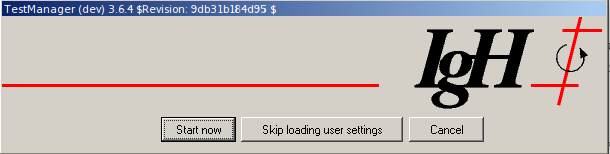
\includegraphics[width=0.5\textwidth]{genpicts/testmanager-00.eps}
\end{center}

It can be closed by clicking on the \textit{Start Now} button,
or by waiting few seconds until the red progression bar reaches
IgH logo at the right side.


\item The main windows appears. Fill the host (127.0.0.1) and port
  (2345) input boxes, then click \textit{Connect}.

\begin{center}
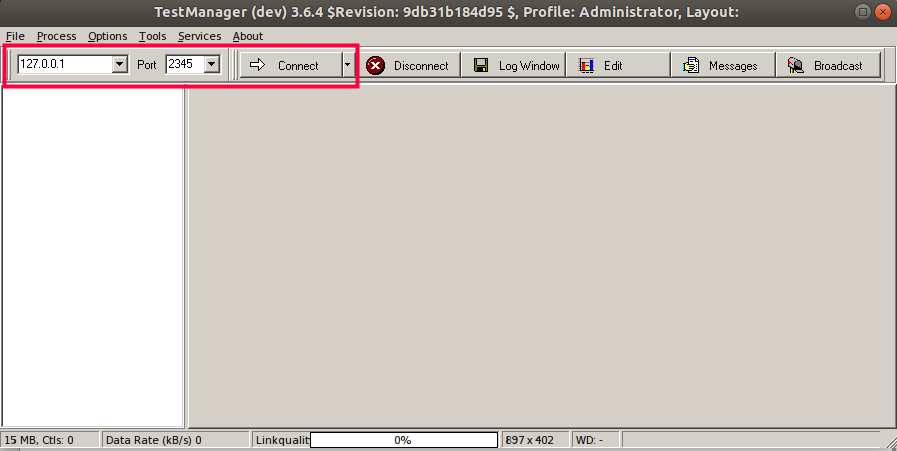
\includegraphics[width=\textwidth]{genpicts/testmanager-01.eps}
\end{center}


\item If the connection is successful, a tree item appears on the left
  side, and the link quality bar becomes green

\begin{center}
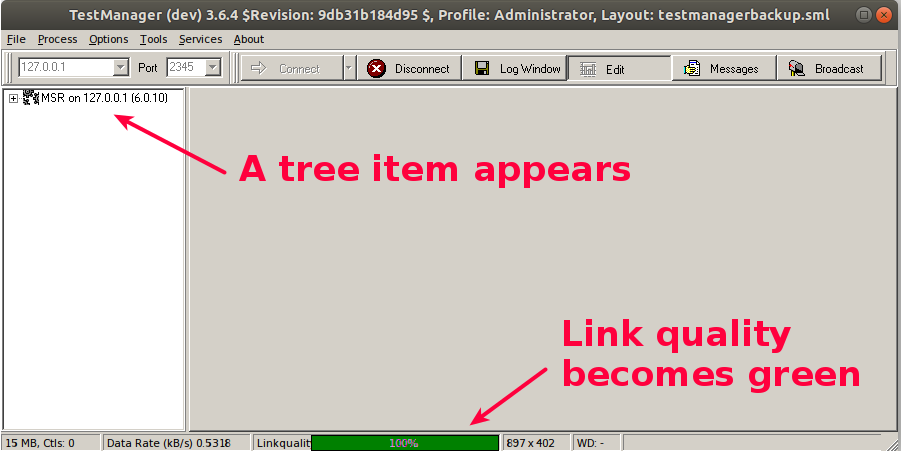
\includegraphics[width=\textwidth]{genpicts/testmanager-02.eps}
\end{center}

If nothing appears, check that the test server\footnote{see
section \ref{test-server-for-testmanager}}
is still running and that the host and port are correctly
typed in the input boxes.


\item Create a widget to display the signal.
  Right-click on the right panel, and select \textit{New Page}.

\begin{center}
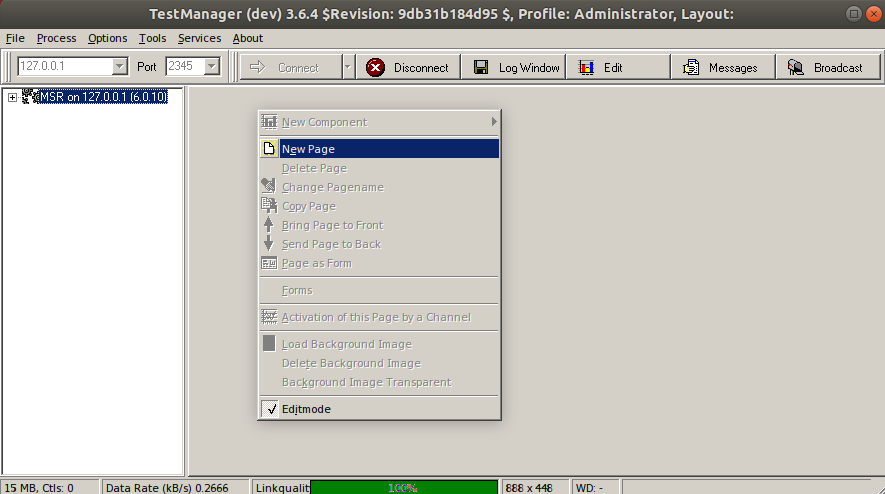
\includegraphics[width=\textwidth]{genpicts/testmanager-03.eps}
\end{center}

\item Enter a page name, for example \textit{Page1}

\begin{center}
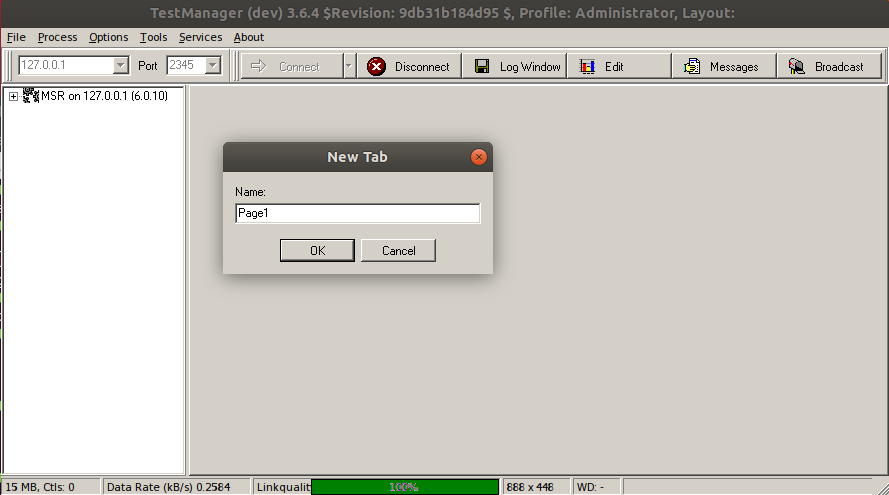
\includegraphics[width=\textwidth]{genpicts/testmanager-04.eps}
\end{center}


\item Right-click on \textit{Page1}, and select \textit{New Component | Channel (Graph) | Single Channell Scrolling Graph}

\begin{center}
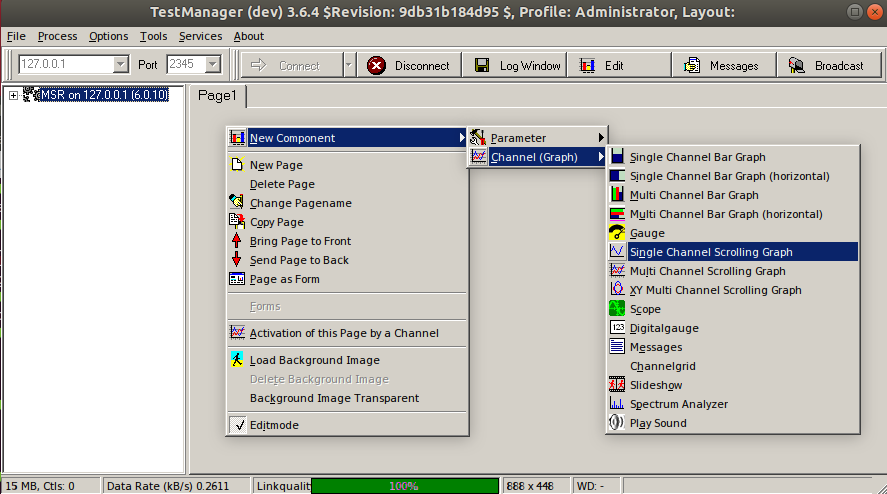
\includegraphics[width=\textwidth]{genpicts/testmanager-05.eps}
\end{center}

\item Expand the tree in the left panel to find the
  \textit{RT-Variable/s1/c}. channel. Drag-and-drop it to the orange area at
  the bottom of the channel widget.

\begin{center}
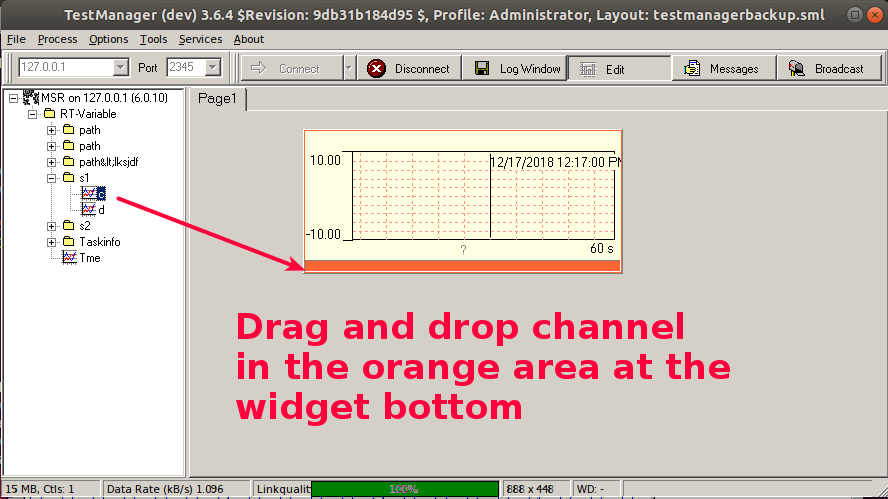
\includegraphics[width=\textwidth]{genpicts/testmanager-06.eps}
\end{center}


\item The channel is plotted in real-time. Drag the corner of the widget to
  increase the size to see better the channel.

\begin{center}
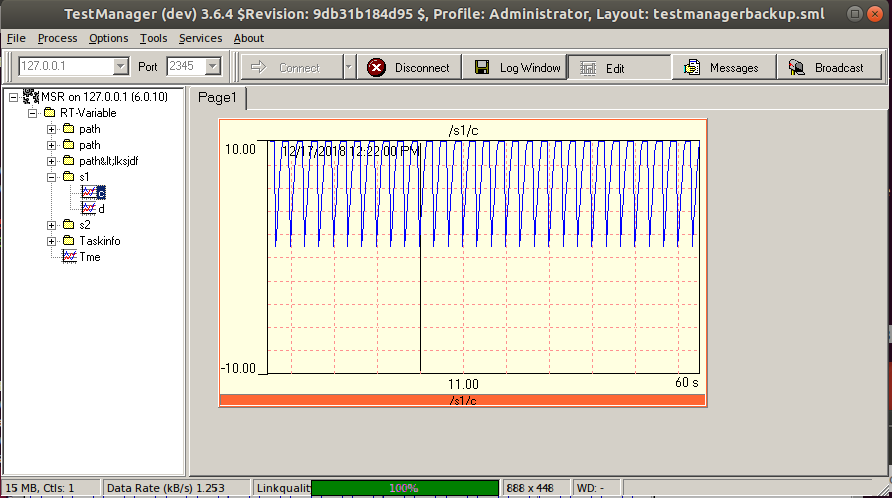
\includegraphics[width=\textwidth]{genpicts/testmanager-07.eps}
\end{center}


\item To edit the widget properties, right-click on it, then select \textit{Configure}

\begin{center}
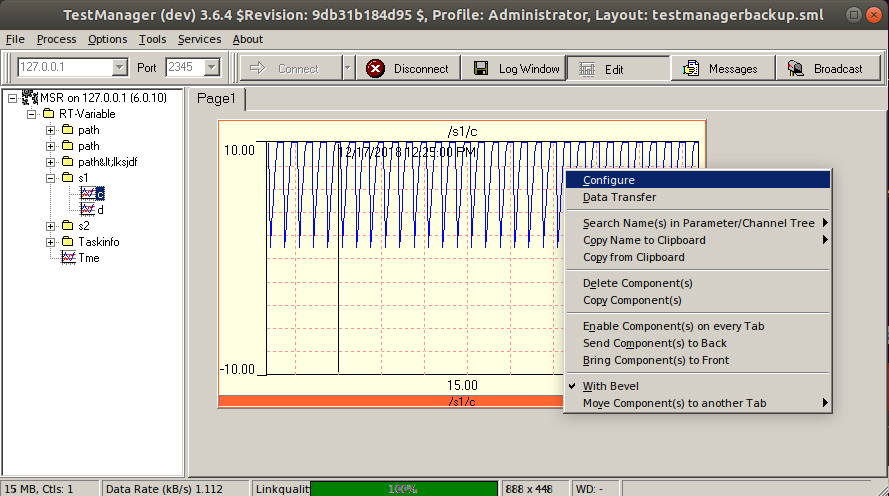
\includegraphics[width=\textwidth]{genpicts/testmanager-08.eps}
\end{center}

The property window appears. Change the following values:
\begin{itemize}
\item Maximal Value = 20
\item Minimum Value = 0
\end{itemize}

\begin{center}
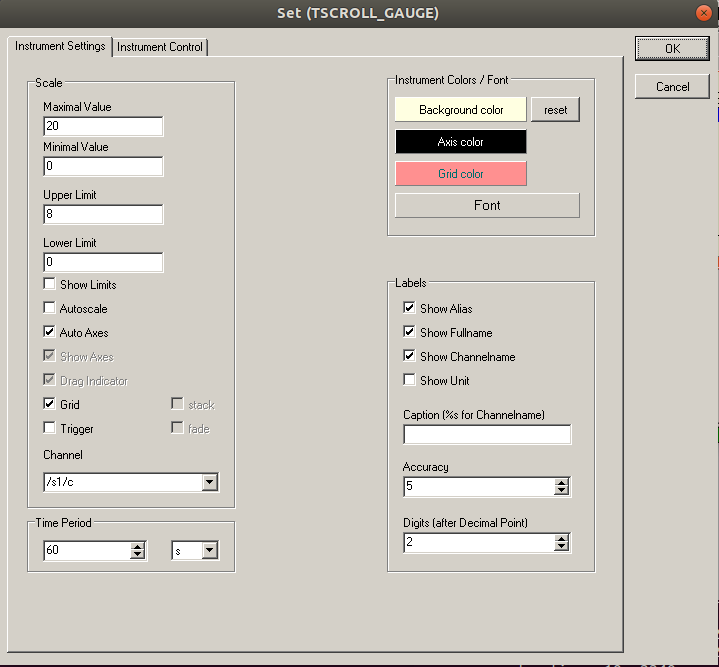
\includegraphics[width=0.7\textwidth]{genpicts/testmanager-09.eps}
\end{center}

\item The default sample rate is low (2~Hz), to increase it,
  right-click on the widget, then select \textit{Data Transfer}

\begin{center}
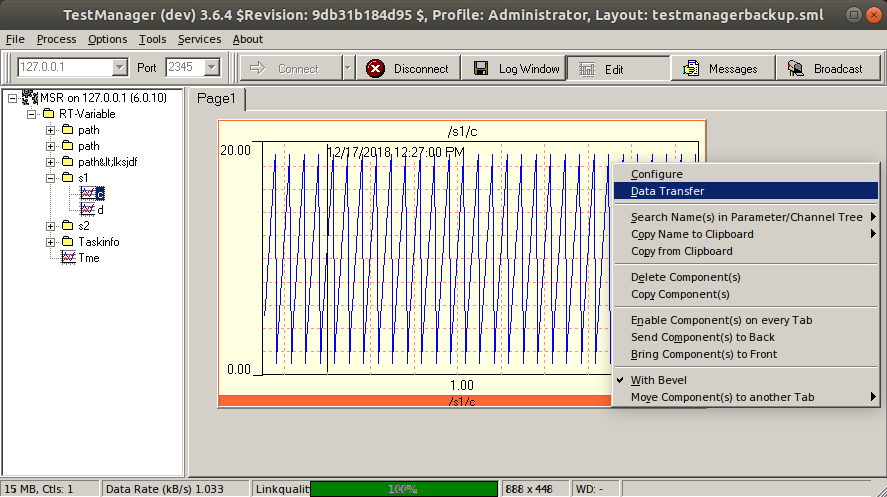
\includegraphics[width=\textwidth]{genpicts/testmanager-10.eps}
\end{center}

The Data Transfer window appears.  To have a smoother
curve, increase both \textit{Sample Rate} and \textit{Buffer Size/s}.
\begin{itemize}
\item Sample Rate = 10
\item Buffer Size /s = 600
\end{itemize}

\begin{center}
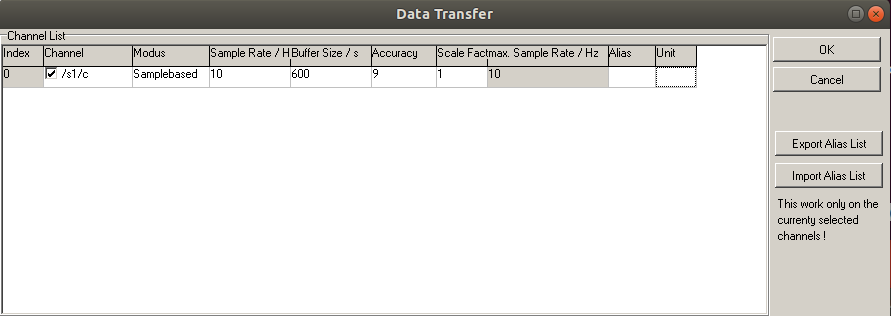
\includegraphics[width=\textwidth]{genpicts/testmanager-11.eps}
\end{center}



\begin{center}
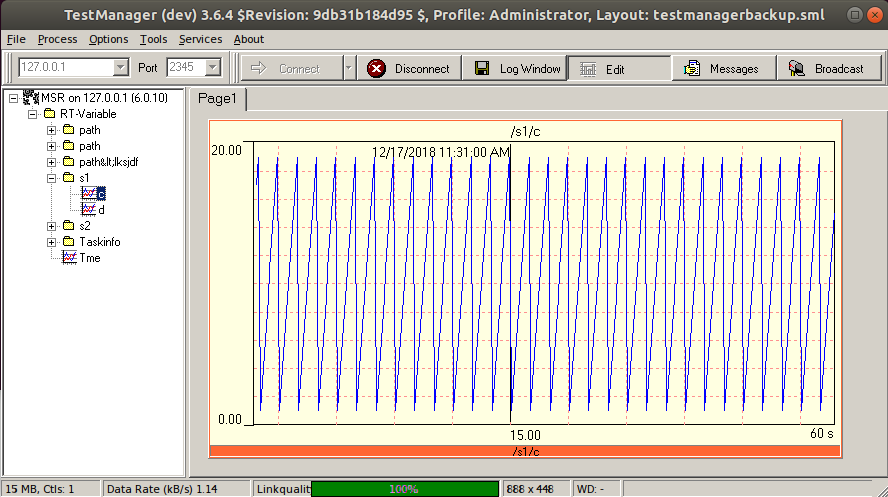
\includegraphics[width=\textwidth]{genpicts/testmanager-12.eps}
\end{center}

\section{Go further}
To go further with Testmanager, you need to read the official
documentation which is available in \cite{testmanager_user_manual}.

\end{itemize}
